\documentclass{article}
\usepackage[utf8]{inputenc}
% Better font encoding for French and scalable fonts
\usepackage[T1]{fontenc}
\usepackage{lmodern}
\usepackage{amsmath, amssymb, amsfonts, amsthm}
\usepackage{graphicx}
\usepackage{booktabs}
\usepackage{geometry}
\usepackage[french]{babel}
\usepackage{amsopn}

\title{Préentraînement auto-supervisé (MAE) sur les TLE SpaceTrack : \\ analyse comparative des runs sur le catalogue LEO}
\author{Etienne Chevrolat}
\date{}


\begin{document}

\maketitle

\begin{abstract}
On rend compte du préentraînement par \textit{masked autoencoder} mené sur l'historique TLE SpaceTrack du catalogue LEO (15\,115 objets, 3\,023 en validation), du premier run du 11 août à la grille d'ablation du 26 août, soit 21 checkpoints exploitables.

Un constat conditionne toute lecture des résultats : \textbf{les val loss de ces runs ne sont pas comparables entre elles}. Le jeu de features a changé le 18 août (11 $\to$ 12 canaux), la pondération de la loss a connu quatre régimes successifs, et la normalisation a changé le 26 août ; à chaque fois la cible change d'échelle ou de composition. Les tailles de fenêtre (48 à 256) et les taux de masquage (0,30 à 0,65) diffèrent en outre d'un run à l'autre, ce qui modifie la difficulté de la tâche indépendamment du modèle.

On construit donc un protocole d'évaluation commun (\texttt{src/scripts/eval\_pretrain.py}) : mêmes objets de validation, mêmes statistiques de normalisation, métriques en unités physiques et rendues invariantes à la longueur de fenêtre. L'erreur de reconstruction y est décomposée en une erreur de \emph{niveau} et une erreur de \emph{forme}, chacune rapportée à la grandeur qui la gouverne. Chaque modèle est évalué à son propre taux de masquage et sur toute la grille des taux, ce qui sépare la difficulté de la tâche de la qualité du modèle. Les tableaux de ce rapport sont générés directement par le script d'évaluation.

Quatre familles de mesures sont rapportées : décomposition de la loss par canal, erreur de reconstruction en kilomètres, restitution des ruptures de niveau du demi-grand axe, et information contenue dans la représentation (sonde linéaire sur embedding gelé, clustering HDBSCAN). Une grille d'ablation à budget égal (200 époques, un facteur modifié à la fois) complète les runs historiques, dont les facteurs sont confondus.

Toute l'implémentation est dans le repo de travail global \texttt{ssa-analysis/}.
\end{abstract}

\section{Objectif et données}

\subsection{Ce que le préentraînement doit produire}

Le préentraînement n'est pas la tâche finale. Il doit fournir une \textbf{représentation par objet} --- le token CLS de l'encodeur, moyenné sur toutes les fenêtres de la série --- qui alimente deux usages en aval :
\begin{itemize}
    \item la \textbf{clusterisation du catalogue LEO} par comportement orbital, par HDBSCAN sur les embeddings ;
    \item la \textbf{détection de manoeuvres}, l'encodeur servant de \textit{backbone} gelé à une tête supervisée entraînée sur manoeuvres labellisées.
\end{itemize}

Ces deux usages portent sur la représentation, non sur la reconstruction. Le rapport mesure donc les deux : les métriques de reconstruction (sections 5.1 à 5.4) et les métriques de représentation (sections 5.7 et 5.8), sans supposer que les premières prédisent les secondes.

\subsection{Le jeu de données}

Historique TLE SpaceTrack du régime LEO : \textbf{15\,115 objets}, à cadence \emph{irrégulière} (médiane de quelques heures, queue au-delà de 24\,h), ce qui interdit l'hypothèse de grille régulière et impose une feature temporelle explicite. Le split est fait \textbf{par objet} (80/20, graine 42), de sorte qu'aucune fenêtre d'un objet de validation n'apparaît à l'entraînement : 12\,092 objets d'entraînement, 3\,023 en validation.

\subsection{Les features}

\vspace{0.3cm}
\noindent\fbox{%
\begin{minipage}{0.98\textwidth}
\textbf{Les douze canaux d'entrée} (\texttt{build\_features}, \texttt{src/ml/datahandler.py})
\begin{enumerate}
    \item \textbf{Temps} : $\Delta t = \log(1 + \delta t)$ entre deux TLE consécutifs, la distribution des écarts étant à queue lourde ;
    \item \textbf{Éléments équinoxiaux} : $k = e\cos\omega$, $h = e\sin\omega$, $p = \tan(i/2)\cos\Omega$, $q = \tan(i/2)\sin\Omega$, plus $\cos M$ et $\sin M$. Ces éléments évitent les singularités à faible excentricité et faible inclinaison, où $\omega$ et $\Omega$ sont mal définis, et sont continus, donc apprenables par un réseau qui n'a aucune notion de périodicité angulaire ;
    \item \textbf{Incréments} : $\Delta a$, $\Delta p$, $\Delta q$ d'un TLE au suivant, qui portent la signature impulsionnelle des manoeuvres ;
    \item \textbf{Décomposition du demi-grand axe} : \texttt{sma\_level} $= \bar{a}$ (moyenne sur l'objet, en km) et \texttt{sma\_local} $= a - \bar{a}$. Cette séparation distingue \emph{où} l'objet orbite de \emph{comment} son orbite évolue.
\end{enumerate}
\end{minipage}
}
\vspace{0.3cm}

La décomposition \texttt{sma\_level} / \texttt{sma\_local} date du 18 août (commit \texttt{796eed0}). Elle isole dans un canal unique la variation du demi-grand axe autour de sa moyenne, ce qui permet de mesurer l'erreur de reconstruction sur cette grandeur séparément du niveau de l'orbite. Les runs antérieurs, à 11 canaux, ne portent pas ce canal et ne sont donc pas ré-évaluables sous le protocole de la section 4.

\section{Architecture}

Masked autoencoder au sens de He \textit{et al.}~\cite{he2022mae}, adapté aux séries temporelles multivariées : la fenêtre est découpée en patchs temporels, une fraction est masquée, \textbf{l'encodeur ne voit que les patchs visibles}, et un décodeur nettement plus léger reconstruit les patchs manquants à partir des tokens encodés et d'un token de masque appris. L'asymétrie encodeur/décodeur et le calcul de la loss \emph{uniquement} sur les patchs masqués viennent directement de ce papier ; l'implémentation est adaptée de VideoMAEv2~\cite{wang2023videomaev2}. Le découpage d'une série multivariée en patchs suit la logique de PatchTST~\cite{nie2023patchtst}.

\begin{center}
\begin{tabular}{lccccc}
\toprule
Modèle & Blocs enc. & Dim. enc. & Blocs déc. & Dim. déc. & Paramètres \\
\midrule
\texttt{miniMAE} & 1 & 32 & 1 & 16 & $\sim$10\,k \\
\texttt{MAEv1} & 4 & 64 & 2 & 32 & 240\,k \\
\texttt{MAEv2} & 12 & 128 & 4 & 64 & 2,6\,M \\
\bottomrule
\end{tabular}
\end{center}

Deux points d'implémentation ont des conséquences directes sur l'analyse :

\paragraph{La projection de sortie n'est supervisée que sur les patchs masqués.} Sur les patchs visibles, \texttt{pred\_space\_proj} n'a jamais reçu de gradient : sa sortie y est arbitraire. Les figures de reconstruction ne tracent donc le prédit que sur les zones masquées, seules interprétables.

\paragraph{La loss est une MSE pondérée par canal} (\texttt{MaskedChannelMSE}), la pondération étant un choix de conception qui a évolué --- et c'est précisément l'un des facteurs qui rendent les runs incomparables.

\subsection{Normalisation par fenêtre}

Les runs du 26 août ajoutent une normalisation par fenêtre inspirée de RevIN~\cite{kim2022revin}, appliquée au seul canal \texttt{sma\_local}. Elle est interne au modèle : la fenêtre est centrée-réduite en entrée de l'encodeur, et \texttt{reconstruct\_window} annule la transformation en sortie, de sorte que l'appelant retrouve la reconstruction dans l'espace du scaler amont.

Pour une fenêtre $b$, en notant $V_b$ l'ensemble des patchs \emph{visibles} et $W$ l'ensemble de tous les points de la fenêtre :
\begin{equation}
\mu_b = \frac{1}{|V_b|\,P}\sum_{(n,t)\in V_b} x_{b,n,t},
\qquad
\sigma_b = \max\Bigl(\; \bigl[\tfrac{1}{|W|}\textstyle\sum_{t\in W}(x_{b,t}-\bar{x}_b)^2\bigr]^{1/2},\; \sigma_{\min} \Bigr),
\qquad
\tilde{x} = \frac{x-\mu_b}{\sigma_b}.
\end{equation}

\paragraph{Les deux statistiques ne sont pas estimées sur le même support, et c'est délibéré.}
\begin{itemize}
    \item $\mu_b$ est estimée sur les \textbf{patchs visibles seulement}. L'estimer sur la fenêtre entière fournirait au décodeur le niveau moyen des patchs masqués, c'est-à-dire précisément la grandeur qu'il doit reconstruire : la mesure d'amélioration serait alors illusoire. Contrôle effectué : en ajoutant $+1000$ aux patchs masqués d'une fenêtre, $\mu_b$ ne varie pas d'une quantité mesurable.
    \item $\sigma_b$ est estimée sur la \textbf{fenêtre entière}. L'estimer sur les seuls patchs visibles conduit à une pathologie mesurée : quand les patchs visibles sont plats, $\sigma_b$ tombe au plancher, et si les patchs masqués contiennent une transition d'orbite, la cible normalisée atteint plusieurs milliers. Sur 2\,400 fenêtres, l'écart-type de la cible passe de $16{,}47$ à $0{,}86$ et son maximum de $1\,988$ à $16$ selon le support d'estimation ; la part de la loss portée par $1\,\%$ des fenêtres passe de $96{,}0\,\%$ à $2{,}5\,\%$. La fuite résiduelle est d'un ordre inférieur à celle du niveau : connaître l'amplitude d'une fenêtre ne renseigne pas sur le profil des patchs masqués.
\end{itemize}

\paragraph{Le plancher $\sigma_{\min}$.} Sans plancher, une fenêtre dont la variation est de l'ordre du bruit d'estimation est ramenée à variance unité, et le modèle est entraîné à reconstruire ce bruit. Le plancher s'exprime dans les unités du scaler amont ; sur LEO, où $\sigma^{\text{scaler}} = 29{,}80$~km pour ce canal, la valeur retenue $\sigma_{\min} = 1{,}3\times10^{-3}$ correspond à $38{,}7$~m.

Les deux erreurs que ce paramètre arbitre vont en sens inverse, et sont mesurées sur $7\,074$ fenêtres de validation :

\begin{center}
\begin{tabular}{cccc}
\toprule
$\sigma_{\min}$ & Équivalent (m) & Fenêtres au plancher & Objets dont le bruit dépasse $\sigma_{\min}$ \\
\midrule
$5{,}0\times10^{-4}$ & 14,9 & 12,6\,\% & 45,6\,\% \\
$1{,}0\times10^{-3}$ & 29,8 & 21,1\,\% & 21,1\,\% \\
\textbf{$1{,}3\times10^{-3}$} & \textbf{38,7} & \textbf{29,8\,\%} & \textbf{11,6\,\%} \\
$1{,}5\times10^{-3}$ & 44,7 & 36,2\,\% & 9,7\,\% \\
$2{,}0\times10^{-3}$ & 59,6 & 48,4\,\% & 8,2\,\% \\
\bottomrule
\end{tabular}
\end{center}

À la valeur retenue, $29{,}8\,\%$ des fenêtres sont clampées ; leur amplitude crête-à-crête réelle vaut $129$~m en médiane et $378$~m au p90, pour un bruit d'estimation médian de $13$~m. Sur ces fenêtres, la normalisation n'est donc pas proportionnelle à leur dispersion propre, et l'échelle effective de la cible reste celle du plancher. C'est une limite connue de la configuration actuelle, dont les résultats des sections 5.3 et 5.4 héritent.

Les deux pourcentages du tableau portent sur des dénominateurs différents --- fenêtres d'un côté, objets de l'autre --- et leur égalité à $\sigma_{\min} = 1{,}0\times10^{-3}$ n'a pas de statut d'optimum ; c'est un repère.

\paragraph{Étendue de la distribution.} L'écart-type par fenêtre de \texttt{sma\_local} sur LEO va de $9$~m au p10 à $19$~km au p90, soit plus de trois ordres de grandeur. C'est cette étendue qui motive une normalisation par fenêtre plutôt qu'un unique facteur d'échelle par canal.

\section{Le problème de comparabilité}

\subsection{Trois ruptures et deux facteurs de difficulté}

\vspace{0.3cm}
\noindent\fbox{%
\begin{minipage}{0.98\textwidth}
\textbf{Pourquoi les val loss ne se comparent pas}
\begin{itemize}
    \item \textbf{18 août --- changement de features} : ajout de \texttt{sma\_level} et \texttt{sma\_local}, 11 $\to$ 12 canaux. La loss porte sur un autre ensemble de cibles ;
    \item \textbf{25 août --- changement des poids} : les trois canaux d'incréments passent à poids nul. La loss porte sur quatre canaux au lieu de sept ;
    \item \textbf{26 août --- changement de normalisation} : normalisation par fenêtre sur \texttt{sma\_local}. La cible change d'échelle ;
    \item \textbf{taille de fenêtre} (48 à 256) et \textbf{taux de masquage} (0,30 à 0,65) : ils changent la \emph{difficulté de la tâche}, pas la qualité du modèle. Reconstruire 30\,\% d'une fenêtre est mécaniquement plus facile que 65\,\%.
\end{itemize}
\end{minipage}
}
\vspace{0.3cm}

Les dix runs antérieurs au 18 août sont de surcroît \textbf{définitivement non ré-évaluables} : le constructeur de features qui les a produits n'existe plus dans le code. Ils ne figurent ici que par leurs courbes loggées.

\subsection{Le protocole commun}

\vspace{0.3cm}
\noindent\fbox{%
\begin{minipage}{0.98\textwidth}
\textbf{Protocole d'évaluation} (\texttt{src/scripts/eval\_pretrain.py})
\begin{enumerate}
    \item \textbf{Mêmes données, même split} : les séries sont chargées une seule fois, le scaler ajusté une seule fois sur le train, et tous les checkpoints sont évalués sur les mêmes objets de validation ;
    \item \textbf{Chaque modèle sur sa propre fenêtre} : les embeddings positionnels sont appris et de longueur fixe, un modèle entraîné en $W=192$ ne peut pas être évalué en $W=256$ ;
    \item \textbf{Métriques invariantes à la longueur de fenêtre} : l'erreur est rapportée par \emph{patch masqué} et découpée par l'amplitude de ce patch, jamais par celle de la fenêtre ;
    \item \textbf{Unités physiques} : l'erreur sur \texttt{sma\_local} est convertie en kilomètres en composant les deux normalisations, celle de la fenêtre (RevIN) et celle du scaler amont ;
    \item \textbf{Double point de fonctionnement} : chaque modèle est évalué à son propre taux de masquage \emph{et} sur toute la grille des taux, ce qui sépare la difficulté de la tâche de la qualité du modèle ;
    \item \textbf{Masquage à graine fixe} : deux évaluations du même checkpoint donnent exactement les mêmes chiffres.
\end{enumerate}
\end{minipage}
}
\vspace{0.3cm}

\paragraph{Contrôle de fidélité.} Le protocole doit retrouver ce que l'entraînement mesurait. Sur le run de référence du 21 août, la loss recalculée vaut $0{,}0479$ contre $0{,}0470$ loggée, soit un écart de $1{,}8\,\%$ --- le split, le scaler et la pondération sont bien ceux de l'entraînement.

\subsection{Séparer l'erreur de forme de l'erreur de niveau}

Une erreur de reconstruction sur un patch se décompose en un \textbf{décalage constant} sur le patch (erreur de niveau) et une \textbf{erreur sur la forme} du signal autour de ce niveau :
$$
\mathrm{MSE} = \underbrace{\overline{\varepsilon}^{\,2}}_{\text{niveau}} + \underbrace{\mathrm{Var}(\varepsilon)}_{\text{forme}}, \qquad \varepsilon = \hat{a} - a .
$$
Ces deux termes ne sont pas gouvernés par la même chose. La forme dépend de l'amplitude locale du signal ; le niveau dépend de la position de l'objet dans sa décroissance, qui peut atteindre la centaine de kilomètres et n'a aucun rapport avec l'agitation locale. Les mélanger produit des non-monotonies dénuées de sens physique : un patch calme appartenant à un objet en décroissance profonde porte un biais énorme et fait exploser la moyenne de son bucket.

\textbf{Ce rapport les mesure donc séparément} : l'erreur de forme contre l'amplitude du patch, l'erreur de niveau contre la magnitude de \texttt{sma\_local}. Cette distinction n'est pas cosmétique --- la normalisation par fenêtre agit spécifiquement sur le second terme.

\section{Métriques}

Cette section définit exactement chaque grandeur rapportée et précise contre quoi elle se lit. Sauf mention contraire, $B$ désigne le nombre de fenêtres évaluées, $N_m$ le nombre de patchs masqués par fenêtre, $F=12$ le nombre de canaux et $P$ le nombre de points par patch. On note $x_{b,n,c,t}$ la cible et $\hat{x}_{b,n,c,t}$ la reconstruction, pour la fenêtre $b$, le patch masqué $n$, le canal $c$ et l'instant $t \in \{1,\dots,P\}$ à l'intérieur du patch. \textbf{Toutes ces grandeurs ne portent que sur les patchs masqués} : la projection de sortie n'est supervisée que sur eux.

\subsection{Loss d'entraînement}

L'erreur quadratique moyenne par canal est
\begin{equation}
d_c^2 = \frac{1}{B\,N_m\,P}\sum_{b=1}^{B}\sum_{n=1}^{N_m}\sum_{t=1}^{P}\bigl(\hat{x}_{b,n,c,t}-x_{b,n,c,t}\bigr)^2 ,
\end{equation}
et la loss est leur moyenne pondérée par le vecteur de poids $w \in \mathbb{R}_+^F$ (\texttt{MaskedChannelMSE}) :
\begin{equation}
\mathcal{L} = \frac{\sum_{c=1}^{F} w_c\, d_c^2}{\sum_{c=1}^{F} w_c}.
\label{eq:loss}
\end{equation}
Un canal de poids nul n'intervient ni au numérateur ni au dénominateur : mettre un canal à zéro ne dilue pas la loss, il le retire de la moyenne. C'est pourquoi $\mathcal{L}$ change de valeur \emph{et} de signification quand $w$ change, et c'est l'une des trois raisons pour lesquelles les runs ne sont pas comparables par leur val loss.

Les quantités $x$ sont exprimées dans l'espace \emph{normalisé} du run : $\mathcal{L}$ n'a donc pas d'unité physique, et sa valeur dépend des statistiques de normalisation.

\subsection{Skill par canal}

Comparer $d_c^2$ entre canaux n'a pas de sens : chaque canal a sa propre dispersion. On rapporte donc l'erreur à la variance de la cible,
\begin{equation}
\mathrm{skill}_c = 1 - \frac{d_c^2}{v_c},
\qquad
v_c = \frac{1}{B}\sum_{b=1}^{B} \frac{1}{N_m P}\sum_{n,t}\bigl(x_{b,n,c,t} - \bar{x}_{b,c}\bigr)^2 ,
\qquad
\bar{x}_{b,c} = \frac{1}{N_m P}\sum_{n,t} x_{b,n,c,t}.
\end{equation}

\paragraph{Contre quoi cela se lit.} $v_c$ est l'erreur qu'obtiendrait un prédicteur constant par fenêtre, qui sortirait $\bar{x}_{b,c}$, c'est-à-dire \textbf{la moyenne des patchs masqués de cette fenêtre}. Ce prédicteur de référence utilise donc une information dont le modèle ne dispose pas : la moyenne de ce qu'il doit deviner. La lecture correcte est :
\begin{itemize}
    \item $\mathrm{skill}_c = 1$ : reconstruction exacte ;
    \item $\mathrm{skill}_c = 0$ : erreur égale à celle d'un prédicteur à qui l'on aurait donné la moyenne de la région masquée ;
    \item $\mathrm{skill}_c < 0$ : erreur supérieure à celle de ce prédicteur \emph{informé}. Ce n'est pas « pire que trivial » : la référence n'est pas accessible au modèle.
\end{itemize}
Cette convention rend les valeurs négatives fréquentes et attendues sur les canaux de faible dispersion ; elles se lisent comme une distance à une borne favorable, pas comme un échec.

\paragraph{Canaux à variance nulle.} \texttt{sma\_level} est constant sur un objet, donc sur toute fenêtre : $v_c = 0$ et le skill n'y est pas défini. Il est marqué comme tel plutôt que reporté.

\subsection{Décomposition niveau / forme}

Sur un patch $(b,n)$ et un canal $c$, posons $\varepsilon_t = \hat{x}_t - x_t$. L'identité biais--variance est exacte :
\begin{equation}
\underbrace{\frac{1}{P}\sum_{t=1}^{P}\varepsilon_t^2}_{\text{erreur totale}^2}
\;=\;
\underbrace{\bar{\varepsilon}^{\,2}}_{\text{niveau}^2}
\;+\;
\underbrace{\frac{1}{P}\sum_{t=1}^{P}\bigl(\varepsilon_t-\bar{\varepsilon}\bigr)^2}_{\text{forme}^2},
\qquad \bar{\varepsilon}=\frac{1}{P}\sum_t \varepsilon_t .
\label{eq:decomp}
\end{equation}
Le premier terme est un décalage constant du patch reconstruit ; le second mesure l'écart de \emph{profil} une fois ce décalage retiré.

\paragraph{Pourquoi les séparer.} Les deux termes ne dépendent pas des mêmes grandeurs. L'erreur de forme est gouvernée par l'agitation locale du signal dans le patch ; l'erreur de niveau est gouvernée par la position de l'objet dans sa décroissance, qui peut atteindre la centaine de kilomètres et n'a aucun lien avec cette agitation. Les additionner produit des non-monotonies dénuées de sens physique : mesuré sur le run du 21 août, le bucket d'amplitude $0{,}5$--$1{,}5$~km affiche une erreur totale de $8{,}39$~km entre deux buckets voisins à $1{,}36$ et $2{,}50$~km, l'écart étant intégralement porté par le terme de niveau.

Ce rapport découpe donc l'erreur de forme par l'amplitude crête-à-crête du patch masqué, et l'erreur de niveau par $\rho_o = \bigl(\frac{1}{L_o}\sum_i \texttt{sma\_local}_{o,i}^2\bigr)^{1/2}$, l'amplitude propre de l'objet $o$ en kilomètres, mesurée sur les \emph{données brutes}. Cette dernière est indépendante du run : sans quoi un modèle à normalisation par fenêtre, dont la cible a sa moyenne retirée, serait découpé selon une grandeur différente des autres.

\subsection{Passage en unités physiques}

L'erreur sur \texttt{sma\_local} est ramenée en kilomètres en composant les deux normalisations traversées :
\begin{equation}
\varepsilon^{\text{km}} = \varepsilon^{\text{norm}} \times \sigma^{\text{fen}}_{b} \times \sigma^{\text{scaler}}_{o},
\end{equation}
où $\sigma^{\text{scaler}}_{o}$ est l'écart-type du scaler amont pour ce canal (global au catalogue, ou propre à l'objet selon le run) et $\sigma^{\text{fen}}_{b}$ celui de la normalisation par fenêtre ($\equiv 1$ quand elle est inactive). C'est cette composition qui rend les runs comparables malgré des normalisations différentes : la loss ne l'est pas, l'erreur en kilomètres l'est.

\subsection{Plancher de bruit des TLE}

La borne d'atteignabilité est le bruit haute fréquence de la série elle-même. Pour une série $x_t$ portant un bruit blanc additif $\epsilon_t$ d'écart-type $\sigma_\epsilon$, la différence seconde $\Delta^2 x_t = x_{t+2}-2x_{t+1}+x_t$ annule toute composante affine et, ses coefficients étant $(1,-2,1)$, vérifie $\mathrm{Var}(\Delta^2 \epsilon) = (1^2+2^2+1^2)\,\sigma_\epsilon^2 = 6\,\sigma_\epsilon^2$. D'où l'estimateur robuste
\begin{equation}
\hat{\sigma}_\epsilon = \frac{1{,}4826 \times \mathrm{MAD}\bigl(\Delta^2 x\bigr)}{\sqrt{6}},
\end{equation}
le facteur $1{,}4826 = 1/\Phi^{-1}(3/4)$ convertissant l'écart absolu médian en écart-type gaussien. Le choix d'un estimateur robuste est délibéré : les manoeuvres produisent de grandes valeurs de $\Delta^2 x$ qui feraient exploser un estimateur par moments.

\paragraph{Ce que cette borne dit et ne dit pas.} $\hat{\sigma}_\epsilon$ majore le bruit d'estimation, puisque toute courbure réelle de la trajectoire y contribue également. Une erreur de reconstruction inférieure à $\hat{\sigma}_\epsilon$ signale que le modèle reproduit une composante que la mesure ne résout pas ; une erreur très supérieure ne dit pas, à elle seule, d'où vient l'écart.

\subsection{Matrice de transfert du masquage}

Chaque modèle est évalué à sept taux de masquage $r \in \{0{,}25;\,0{,}30;\,0{,}40;\,0{,}45;\,0{,}50;\,0{,}65;\,0{,}80\}$. La grille contient tous les taux d'entraînement rencontrés, de sorte que chaque modèle y figure à son propre point de fonctionnement. La grandeur reportée est l'erreur de forme en kilomètres sur \texttt{sma\_local}.

Une lecture \emph{en ligne} donne la sensibilité d'un modèle au taux d'évaluation ; une lecture \emph{en colonne} compare les modèles à difficulté fixée. Cette dernière est la seule comparaison valide entre modèles entraînés à des taux différents : le taux d'entraînement change la difficulté de la tâche indépendamment de la qualité du modèle, puisque le nombre de points à deviner par point observé en dépend directement.

\paragraph{Réserve.} Évaluer un modèle loin de son taux d'entraînement le place hors de sa distribution d'entrée : le nombre de tokens visibles reçus par l'encodeur diffère de celui vu à l'apprentissage. Une dégradation hors diagonale mélange donc perte de qualité intrinsèque et effet de distribution, et ces deux causes ne sont pas séparées ici.

\subsection{Restitution des ruptures de niveau}

On détecte les ruptures sur \texttt{sma\_local} par différence de médianes glissantes de demi-largeur $k=4$,
\begin{equation}
\delta_t = \mathrm{med}\bigl(x_{t},\dots,x_{t+k-1}\bigr) - \mathrm{med}\bigl(x_{t-k},\dots,x_{t-1}\bigr),
\end{equation}
en retenant les $t$ tels que $|\delta_t| > \max(0{,}15~\text{km},\; 5\,\hat{\sigma}_\epsilon)$, puis en ne gardant qu'un évènement par groupe contigu (le plus fort). Le patch qui contient l'évènement est ensuite \textbf{masqué de force}, les autres patchs masqués étant tirés au hasard de façon à conserver le taux de masquage nominal.

L'amplitude vraie $d^{\text{vrai}}$ et l'amplitude reconstruite $d^{\text{pred}}$ sont mesurées de la même façon, par différence des médianes des deux moitiés du patch. On rapporte la pente de la régression \emph{sans constante}
\begin{equation}
\beta = \frac{\sum_j d^{\text{vrai}}_j\, d^{\text{pred}}_j}{\sum_j \bigl(d^{\text{vrai}}_j\bigr)^2},
\end{equation}
la corrélation de Pearson entre les deux, et la fraction de signes concordants.

\paragraph{Lecture.} $\beta = 1$ correspond à une restitution exacte de l'amplitude ; $\beta = 0$ à $d^{\text{pred}} \equiv 0$, c'est-à-dire au comportement d'une interpolation lisse qui traverse la rupture sans la marquer. La fraction de signes concordants vaut $1/2$ pour une prédiction sans information sur le sens de la rupture.

\paragraph{Deux réserves.} $d^{\text{vrai}}$ est lui-même mesuré avec erreur ; il s'agit d'une régression à variable explicative bruitée, dont la pente est atténuée vers zéro. Le $\beta$ rapporté est donc une borne inférieure de la restitution réelle. Par ailleurs $\beta$ est dominé par les évènements de grande amplitude, d'où le découpage par bucket qui l'accompagne.

\subsection{Sonde linéaire sur embedding gelé}

Protocole standard d'évaluation d'une représentation auto-supervisée~\cite{he2022mae} : l'encodeur est \emph{gelé}, on n'entraîne qu'une régression linéaire de son embedding vers une grandeur physique connue. La représentation d'un objet est le token CLS moyenné sur toutes les fenêtres de sa série. On ajuste une régression ridge ($\alpha = 1$, embeddings centrés-réduits) sur $80\,\%$ des objets et on rapporte, sur les $20\,\%$ restants,
\begin{equation}
R^2 = 1 - \frac{\sum_i (y_i - \hat{y}_i)^2}{\sum_i (y_i - \bar{y})^2},
\end{equation}
$\bar{y}$ étant la moyenne \emph{sur le sous-ensemble de validation}. $R^2 < 0$ signifie une erreur supérieure à celle du prédicteur constant $\bar{y}$.

\paragraph{Transformation des cibles.} L'amplitude du demi-grand axe, la dérive et le bruit propre s'étalent sur plusieurs ordres de grandeur. Sur des cibles brutes, quelques objets à décroissance rapide dominent la somme des carrés et le $R^2$ devient instable : mesuré, il passe de $-0{,}07$ à $-16{,}7$ pour la même quantité selon que l'échantillon compte 600 ou 2000 objets. Ces cibles sont donc compressées par $y \mapsto \log(1+y)$, et $y \mapsto \mathrm{sgn}(y)\log(1+|y|)$ pour la dérive, qui change de signe. On rapporte en complément le coefficient de \textbf{Spearman} $\rho$, corrélation de Pearson des rangs, invariant par transformation monotone et insensible à la queue de distribution : un écart marqué entre $R^2$ et $\rho$ signale que le score dépend de quelques points extrêmes.

\paragraph{Deux familles de cibles, à ne pas confondre.}
\begin{itemize}
    \item \textbf{Contrôle} --- \texttt{sma} moyen, excentricité, inclinaison. Ces grandeurs sont \emph{directement présentes en entrée} : \texttt{sma\_level} est un canal, et $e = \sqrt{k^2+h^2}$, $i = 2\arctan\sqrt{p^2+q^2}$ se déduisent des canaux équinoxiaux par une moyenne sur la fenêtre. Un $R^2$ élevé y vérifie seulement que le CLS retient la moyenne de ce qu'il voit. C'est un test de non-régression, pas une performance.
    \item \textbf{Dynamique} --- dérive du demi-grand axe, amplitude de sa variation, taux de rupture, bruit propre. Ces grandeurs décrivent le comportement de l'objet et ne sont jamais fournies telles quelles.
\end{itemize}

\subsection{Structure de la représentation}

HDBSCAN~\cite{campello2013} est appliqué aux embeddings centrés-réduits à hyperparamètres \textbf{fixés} (\texttt{min\_cluster\_size} $=$ \texttt{min\_samples} $= 15$), identiques pour tous les runs : les laisser s'ajuster par run rendrait les comptages incomparables. On rapporte le nombre de clusters, la fraction d'objets étiquetés bruit (label $-1$), et le coefficient de silhouette moyen sur les seuls objets clusterisés,
\begin{equation}
s(i) = \frac{b(i)-a(i)}{\max\bigl(a(i),b(i)\bigr)} \in [-1,1],
\end{equation}
où $a(i)$ est la distance moyenne de $i$ aux points de son cluster et $b(i)$ le minimum, sur les autres clusters, de la distance moyenne de $i$ à leurs points.

\paragraph{Réserve.} Ces trois grandeurs décrivent la \emph{géométrie} des embeddings, pas leur pertinence : un partitionnement net selon une variable sans intérêt opérationnel donnerait une bonne silhouette. Elles se lisent conjointement avec la sonde linéaire, qui dit \emph{quelle} information est présente.

\section{Résultats}

Les tableaux de cette section sont écrits directement par \texttt{src/scripts/eval\_pretrain.py} dans \texttt{rapport/figures/} et inclus tels quels : aucun chiffre n'est recopié à la main. Les valeurs correspondent à $400$ objets de validation, $8$ fenêtres par objet réparties sur la série, masquage à graine fixe.

\subsection{Inventaire des runs ré-évaluables}

\begin{center}\small
\begin{tabular}{lccccrr}
\toprule
Run & Fenêtre & Patch & Masquage & Blocs & Époques & Val loss \\
\midrule
2026-08-18\_15-41-40 & 192 & 12 & 0,50 & 12 & 193 & 0,1017 \\
2026-08-19\_10-47-37 & 48 & 6 & 0,50 & 12 & 107 & 0,1152 \\
2026-08-20\_16-11-40 & 96 & 12 & 0,30 & 12 & 500 & 0,1035 \\
2026-08-21\_15-21-02 & 256 & 8 & 0,65 & 12 & 500 & 0,0469 \\
2026-08-26\_12-28-30 & 256 & 8 & 0,65 & 12 & 500 & 0,0724 \\
2026-08-26\_13-42-27 & 256 & 8 & 0,65 & 12 & 200 & 0,0732 \\
2026-08-26\_16-02-17 & 192 & 8 & 0,65 & 12 & 200 & 0,0788 \\
2026-08-26\_17-57-08 & 256 & 4 & 0,50 & 12 & 281 & 0,0651 \\
2026-08-26\_17-59-02 & 256 & 4 & 0,65 & 12 & 200 & 0,0656 \\
2026-08-26\_22-28-01 & 256 & 16 & 0,65 & 12 & 196 & 0,0802 \\
\bottomrule
\end{tabular}

\end{center}

Les dix runs antérieurs au 18 août portent 11 canaux et ne figurent pas ici : le constructeur de features qui les a produits n'existe plus dans le code, ils ne sont pas reproductibles. Les runs de moins de 100 époques sont écartés des comparaisons et la liste des exclus est journalisée à l'exécution.

\subsection{Reconstitution de la pondération de chaque run}

La pondération $w$ de l'équation~\eqref{eq:loss} n'a été exposée dans la configuration qu'à partir du 25 août ; avant, elle était codée en dur dans \texttt{train.py} et, pour partie, jamais commitée. Elle n'est donc pas récupérable depuis les artefacts d'un run antérieur. Quatre régimes se sont succédé :

\begin{enumerate}
    \item $w_{\texttt{dt}} = 0$, tout le reste à $1$ ;
    \item $w_{\texttt{dt}} = w_{\cos M} = w_{\sin M} = w_{\texttt{sma\_level}} = 0$, le reste à $1$ ;
    \item idem, plus $w_{\texttt{p\_diff}} = w_{\texttt{q\_diff}} = 0{,}25$ ;
    \item idem, plus $w_{\texttt{sma\_diff}} = w_{\texttt{p\_diff}} = w_{\texttt{q\_diff}} = 0$, ne laissant que $k, h, p, q, \texttt{sma\_local}$.
\end{enumerate}

On calcule la loss du checkpoint sous chacun des quatre et on retient celui qui reproduit la valeur loggée :

\begin{center}\footnotesize
\begin{tabular}{lccccccc}
\toprule
Run & Loggée & 1. dt seul a 0 & 2. + cosM, sinM, sma\_level a 0 & 3. + p\_diff, q\_diff a 0.25 & 4. + increments a 0 & config du run & Retenu \\
\midrule
MAEv2 W192 P12 m0.50 [08-18, 193 ep] & 0,1017 & 0,3469 & 0,1285 & 0,0568 & 0,0027 & 2. + cosM, s \\
MAEv2 W96 P12 m0.30 & 0,1035 & 0,3487 & 0,1298 & 0,0547 & 0,0012 & 2. + cosM, s \\
MAEv2 W256 P8 m0.65 & 0,0469 & 0,3429 & 0,1206 & 0,0498 & 0,0018 & 3. + p\_diff \\
MAEv2 W256 P8 m0.65 revin-fen [08-26, 500 ep] & 0,0724 & 0,4912 & 0,3248 & 0,1660 & 0,0797 & 0,0797 & 4. + increme \\
MAEv2 W256 P8 m0.65 revin-fen [08-26, 200 ep] & 0,0732 & 0,5128 & 0,3381 & 0,1767 & 0,0812 & 0,0812 & 4. + increme \\
MAEv2 W192 P8 m0.65 revin-fen & 0,0788 & 0,5123 & 0,3444 & 0,1814 & 0,0859 & 0,0859 & 4. + increme \\
MAEv2 W256 P4 m0.50 revin-fen & 0,0651 & 0,4914 & 0,3240 & 0,1621 & 0,0728 & 0,0728 & 4. + increme \\
MAEv2 W256 P4 m0.65 revin-fen & 0,0656 & 0,5095 & 0,3256 & 0,1668 & 0,0726 & 0,0726 & 4. + increme \\
MAEv2 W256 P16 m0.65 revin-fen & 0,0802 & 0,5129 & 0,3444 & 0,1798 & 0,0866 & 0,0866 & 4. + increme \\
\bottomrule
\end{tabular}

\end{center}

\paragraph{Ce que cette table établit.} Les régimes 1 et 4 sont écartés pour les runs du 18 au 21 août par un facteur $2{,}4$ à $7$, très au-delà de toute incertitude d'échantillonnage. Le run du 21 août est identifié en régime 3 à $6{,}2\,\%$ près. Les runs à normalisation par fenêtre sont identifiés en régime 4, ce que leur configuration confirme indépendamment.

\paragraph{Ce qu'elle n'établit pas.} Départager les régimes 2 et 3 pour les runs du 18 au 20 août. Les écarts résiduels y sont de $+25\,\%$ à $+39\,\%$ pour le régime 2 et de $-29\,\%$ à $-47\,\%$ pour le régime 3, du même ordre de grandeur que le biais d'échantillonnage du protocole : celui-ci prend $8$ fenêtres par objet réparties sur la série là où l'entraînement en prend une tous les $31$ pas, ce qui sur-pondère les séries courtes. Ces trois runs sont donc rapportés comme « régime 2 ou 3 ».

\subsection{Décomposition de la loss par canal}

Skill par canal, au sens de la section 4.2 --- $0$ correspond à un prédicteur qui connaîtrait la moyenne de la région masquée :

\begin{center}\tiny
\begin{tabular}{lccccccccccc}
\toprule
Run & \texttt{dt} & \texttt{k} & \texttt{h} & \texttt{p} & \texttt{q} & \texttt{cosM} & \texttt{sinM} & \texttt{sma\_diff} & \texttt{q\_diff} & \texttt{p\_diff} & \texttt{sma\_local} \\
\midrule
MAEv2 W192 P12 m0.50 [08-18, 193 ep] & -0,03 & 0,98 & 0,98 & 0,99 & 0,99 & -0,35 & -3,42 & 0,18 & 0,54 & 0,53 & 0,96 \\
MAEv2 W96 P12 m0.30 & -0,06 & 0,93 & 0,93 & 0,99 & 0,99 & -0,98 & -5,53 & 0,51 & 0,38 & 0,40 & 0,95 \\
MAEv2 W256 P8 m0.65 & -0,02 & 0,99 & 0,99 & 0,99 & 0,99 & -0,19 & -2,79 & 0,32 & 0,55 & 0,55 & 0,98 \\
MAEv2 W256 P8 m0.65 revin-fen [08-26, 500 ep] & -0,02 & 0,99 & 1,00 & 0,99 & 0,99 & -0,20 & -2,77 & -0,17 & -0,06 & -0,06 & 0,51 \\
MAEv2 W256 P8 m0.65 revin-fen [08-26, 200 ep] & -0,07 & 0,99 & 0,99 & 0,99 & 0,99 & -0,28 & -2,88 & -0,50 & -0,09 & -0,08 & 0,50 \\
MAEv2 W192 P8 m0.65 revin-fen & -0,06 & 0,99 & 0,99 & 0,99 & 0,99 & -0,36 & -3,28 & -0,38 & -0,10 & -0,07 & 0,46 \\
MAEv2 W256 P4 m0.50 revin-fen & -0,02 & 0,99 & 0,99 & 1,00 & 1,00 & -0,20 & -2,80 & -0,13 & -0,07 & -0,07 & 0,58 \\
MAEv2 W256 P4 m0.65 revin-fen & -0,08 & 1,00 & 1,00 & 1,00 & 1,00 & -0,27 & -3,24 & -0,40 & -0,04 & -0,06 & 0,55 \\
MAEv2 W256 P16 m0.65 revin-fen & -0,04 & 0,99 & 0,99 & 0,99 & 0,99 & -0,25 & -3,03 & -0,34 & -0,11 & -0,12 & 0,46 \\
\bottomrule
\end{tabular}

\end{center}

Part de chaque canal dans la loss pondérée, en pourcentage :

\begin{center}\tiny
\begin{tabular}{lccccccccccc}
\toprule
Run & \texttt{dt} & \texttt{k} & \texttt{h} & \texttt{p} & \texttt{q} & \texttt{cosM} & \texttt{sinM} & \texttt{sma\_diff} & \texttt{q\_diff} & \texttt{p\_diff} & \texttt{sma\_local} \\
\midrule
MAEv2 W192 P12 m0.50 [08-18, 193 ep] & 0,0 & 0,2 & 0,3 & 0,6 & 0,7 & 0,0 & 0,0 & 36,8 & 28,8 & 30,8 & 1,8 \\
MAEv2 W96 P12 m0.30 & 0,0 & 0,2 & 0,1 & 0,4 & 0,3 & 0,0 & 0,0 & 34,3 & 31,5 & 32,6 & 0,7 \\
MAEv2 W256 P8 m0.65 & 0,0 & 0,1 & 0,2 & 0,6 & 0,6 & 0,0 & 0,0 & 31,3 & 32,6 & 33,3 & 1,2 \\
MAEv2 W256 P8 m0.65 revin-fen [08-26, 500 ep] & 0,0 & 0,1 & 0,1 & 0,5 & 0,5 & 0,0 & 0,0 & 0,0 & 0,0 & 0,0 & 98,8 \\
MAEv2 W256 P8 m0.65 revin-fen [08-26, 200 ep] & 0,0 & 0,1 & 0,1 & 0,6 & 0,6 & 0,0 & 0,0 & 0,0 & 0,0 & 0,0 & 98,6 \\
MAEv2 W192 P8 m0.65 revin-fen & 0,0 & 0,1 & 0,1 & 0,6 & 0,6 & 0,0 & 0,0 & 0,0 & 0,0 & 0,0 & 98,6 \\
MAEv2 W256 P4 m0.50 revin-fen & 0,0 & 0,1 & 0,1 & 0,3 & 0,2 & 0,0 & 0,0 & 0,0 & 0,0 & 0,0 & 99,3 \\
MAEv2 W256 P4 m0.65 revin-fen & 0,0 & 0,1 & 0,1 & 0,3 & 0,3 & 0,0 & 0,0 & 0,0 & 0,0 & 0,0 & 99,2 \\
MAEv2 W256 P16 m0.65 revin-fen & 0,0 & 0,1 & 0,1 & 1,1 & 1,1 & 0,0 & 0,0 & 0,0 & 0,0 & 0,0 & 97,5 \\
\bottomrule
\end{tabular}

\end{center}

\paragraph{Lecture.} Sur les runs des régimes 2 et 3, les trois canaux d'incréments concentrent l'essentiel de la loss pondérée tandis que \texttt{sma\_local} en représente moins de $2\,\%$ ; sur les runs du régime 4, où les incréments sont à poids nul, \texttt{sma\_local} en représente plus de $95\,\%$. Les canaux équinoxiaux $k, h, p, q$ ont un skill compris entre $0{,}86$ et $0{,}99$ selon les runs, la valeur la plus basse étant celle de la configuration $W{=}48$, $P{=}6$ ; les quatre autres configurations sont toutes au-dessus de $0{,}92$. Le canal \texttt{sma\_diff} a un skill compris entre $-0{,}22$ et $+0{,}51$ selon les runs, pour une variance de cible de l'ordre de $0{,}12$ en unités normalisées.

\subsection{Erreur de reconstruction en unités physiques}

Erreur de \emph{forme} sur \texttt{sma\_local} en kilomètres, par amplitude crête-à-crête du patch masqué, chaque modèle évalué à son propre taux de masquage :

\begin{center}\small
\begin{tabular}{lcccccc}
\toprule
Run & 0-0.05 & 0.05-0.15 & 0.15-0.5 & 0.5-1.5 & 1.5-5 & >5 \\
\midrule
MAEv2 W192 P12 m0.50 [08-18, 193 ep] & 0,068 & 0,159 & 0,326 & 0,475 & 0,929 & 3,645 \\
MAEv2 W96 P12 m0.30 & 0,082 & 0,080 & 0,200 & 0,287 & 0,825 & 2,960 \\
MAEv2 W256 P8 m0.65 & 0,088 & 0,151 & 0,283 & 0,402 & 0,791 & 2,726 \\
MAEv2 W256 P8 m0.65 revin-fen [08-26, 500 ep] & 0,098 & 0,163 & 0,329 & 0,797 & 0,800 & 2,916 \\
MAEv2 W256 P8 m0.65 revin-fen [08-26, 200 ep] & 0,105 & 0,182 & 0,360 & 0,844 & 0,824 & 3,135 \\
MAEv2 W192 P8 m0.65 revin-fen & 0,105 & 0,212 & 0,373 & 0,680 & 0,867 & 3,360 \\
MAEv2 W256 P4 m0.50 revin-fen & 0,102 & 0,174 & 0,265 & 0,497 & 0,878 & 2,969 \\
MAEv2 W256 P4 m0.65 revin-fen & 0,085 & 0,174 & 0,292 & 0,460 & 0,902 & 2,918 \\
MAEv2 W256 P16 m0.65 revin-fen & 0,155 & 0,222 & 0,504 & 1,005 & 0,958 & 4,458 \\
\bottomrule
\end{tabular}

\end{center}

\begin{center}
    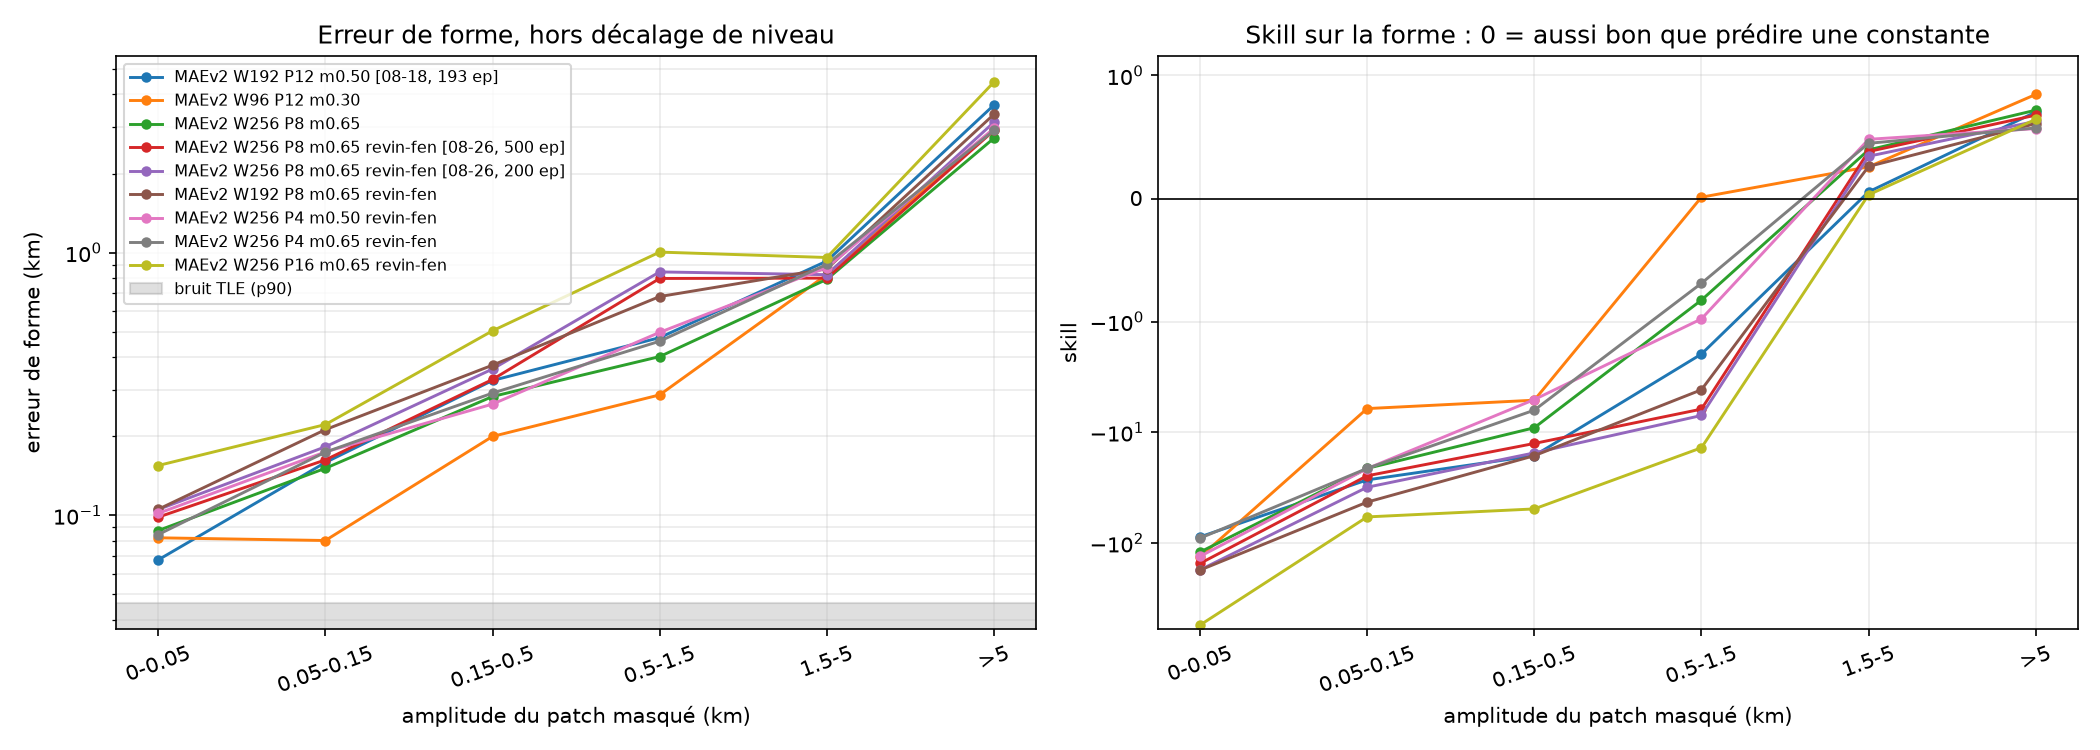
\includegraphics[width=0.98\textwidth]{figures/pretrain_leo_km_error.png}
\end{center}

La bande grise du panneau de gauche marque le p90 du plancher de bruit des TLE mesuré sur les objets de validation ($46$~m ; médiane $13$~m). Le panneau de droite porte le skill en échelle symlog, la référence étant un prédicteur qui connaîtrait la moyenne du patch masqué.

\subsection{Matrice de transfert du taux de masquage}

\begin{center}\footnotesize
\begin{tabular}{lccccccc}
\toprule
Run & 0,25 & 0,30 & 0,40 & 0,45 & 0,50 & 0,65 & 0,80 \\
\midrule
MAEv2 W192 P12 m0.50 [08-18, 193 ep] & 0,639 & 0,659 & 0,672 & 0,733 & \textbf{0,940} & 0,960 & 1,140 \\
MAEv2 W96 P12 m0.30 & 0,644 & \textbf{0,644} & 0,728 & 1,097 & 1,097 & 1,569 & 2,836 \\
MAEv2 W256 P8 m0.65 & 0,440 & 0,462 & 0,488 & 0,486 & 0,494 & \textbf{0,532} & 0,646 \\
MAEv2 W256 P8 m0.65 revin-fen [08-26, 500 ep] & 0,544 & 0,561 & 0,580 & 0,567 & 0,558 & \textbf{0,632} & 0,807 \\
MAEv2 W256 P8 m0.65 revin-fen [08-26, 200 ep] & 0,661 & 0,657 & 0,660 & 0,642 & 0,636 & \textbf{0,706} & 0,841 \\
MAEv2 W192 P8 m0.65 revin-fen & 0,787 & 0,751 & 0,730 & 0,713 & 0,708 & \textbf{0,743} & 0,871 \\
MAEv2 W256 P4 m0.50 revin-fen & 0,498 & 0,478 & 0,453 & 0,440 & \textbf{0,439} & 0,484 & 1,020 \\
MAEv2 W256 P4 m0.65 revin-fen & 0,527 & 0,499 & 0,453 & 0,437 & 0,429 & \textbf{0,404} & 0,501 \\
MAEv2 W256 P16 m0.65 revin-fen & 0,979 & 0,937 & 0,927 & 0,985 & 1,135 & \textbf{1,090} & 1,679 \\
\bottomrule
\end{tabular}

\end{center}

\begin{center}
    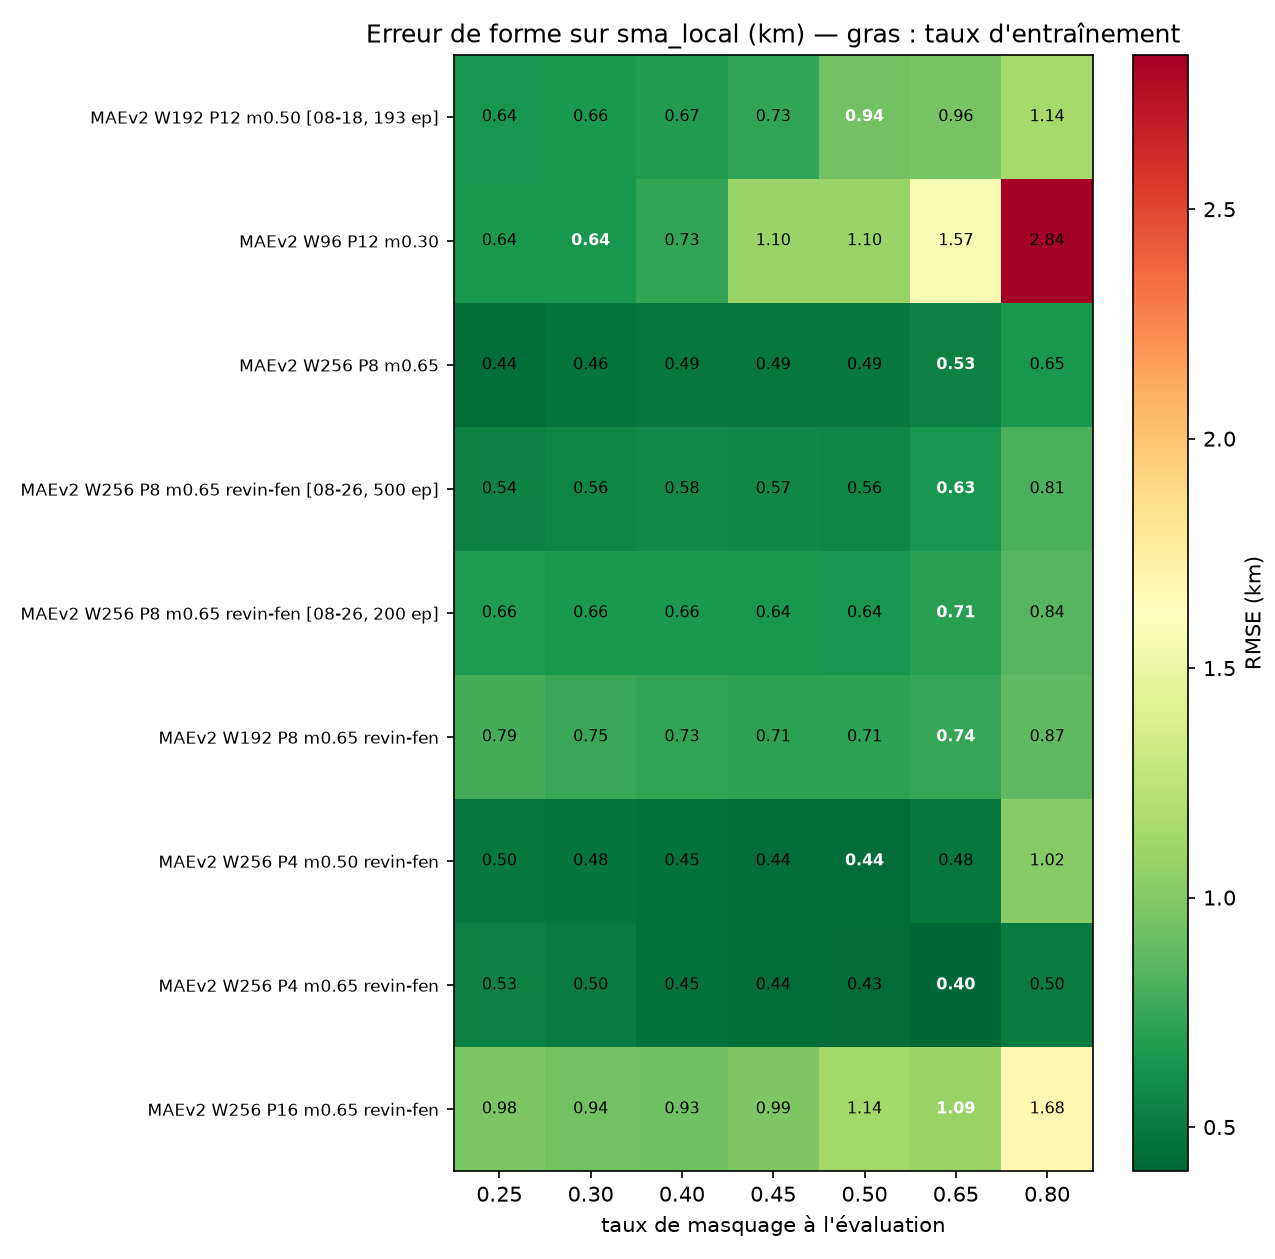
\includegraphics[width=0.86\textwidth]{figures/pretrain_leo_mask_matrix.png}
\end{center}

\paragraph{Lecture en colonne, à difficulté fixée.} La configuration $W{=}256$, $P{=}8$, masquage $0{,}65$ présente l'erreur de forme la plus faible aux \emph{sept} taux d'évaluation, de $0{,}440$~km à $r=0{,}25$ à $0{,}646$~km à $r=0{,}80$. L'écart avec les autres configurations n'est donc pas imputable à une différence de difficulté de la tâche d'entraînement.

\paragraph{Lecture en ligne, sensibilité au taux.} Le modèle entraîné à $0{,}30$ voit son erreur passer de $0{,}64$~km à $2{,}84$~km entre les taux d'évaluation $0{,}25$ et $0{,}80$, soit un facteur $4{,}4$ ; celui entraîné à $0{,}65$ passe de $0{,}44$ à $0{,}65$~km, soit un facteur $1{,}5$. La réserve de la section 4.6 s'applique : cet écart mélange qualité intrinsèque et effet de distribution d'entrée.

\subsection{Restitution des ruptures de niveau}

Pente $\beta$ de la régression sans constante de l'amplitude reconstruite sur l'amplitude vraie, globale puis par bucket d'amplitude. $\beta = 1$ correspond à une restitution exacte, $\beta = 0$ au comportement d'une interpolation lisse.

\begin{center}\footnotesize
\begin{tabular}{lccccc}
\toprule
Run & Global & 0.05-0.2 & 0.2-0.5 & 0.5-1.5 & >1.5 \\
\midrule
MAEv2 W192 P12 m0.50 [08-18, 193 ep] & 0,72 & 3,50 & 2,24 & 2,04 & 0,71 \\
MAEv2 W96 P12 m0.30 & 0,97 & 2,66 & 2,20 & 1,31 & 0,97 \\
MAEv2 W256 P8 m0.65 & 0,67 & 1,24 & 3,35 & 1,39 & 0,66 \\
MAEv2 W256 P8 m0.65 revin-fen [08-26, 500 ep] & 0,54 & 1,31 & 2,36 & 1,33 & 0,54 \\
MAEv2 W256 P8 m0.65 revin-fen [08-26, 200 ep] & 0,49 & 1,30 & 2,90 & 1,42 & 0,49 \\
MAEv2 W192 P8 m0.65 revin-fen & 0,56 & 2,05 & 2,81 & 1,56 & 0,56 \\
MAEv2 W256 P4 m0.50 revin-fen & 0,58 & 0,99 & 0,93 & 1,03 & 0,57 \\
MAEv2 W256 P4 m0.65 revin-fen & 0,58 & 0,65 & 0,85 & 1,10 & 0,58 \\
MAEv2 W256 P16 m0.65 revin-fen & 0,68 & 3,27 & 2,53 & 3,27 & 0,68 \\
\bottomrule
\end{tabular}

\end{center}

\begin{center}
    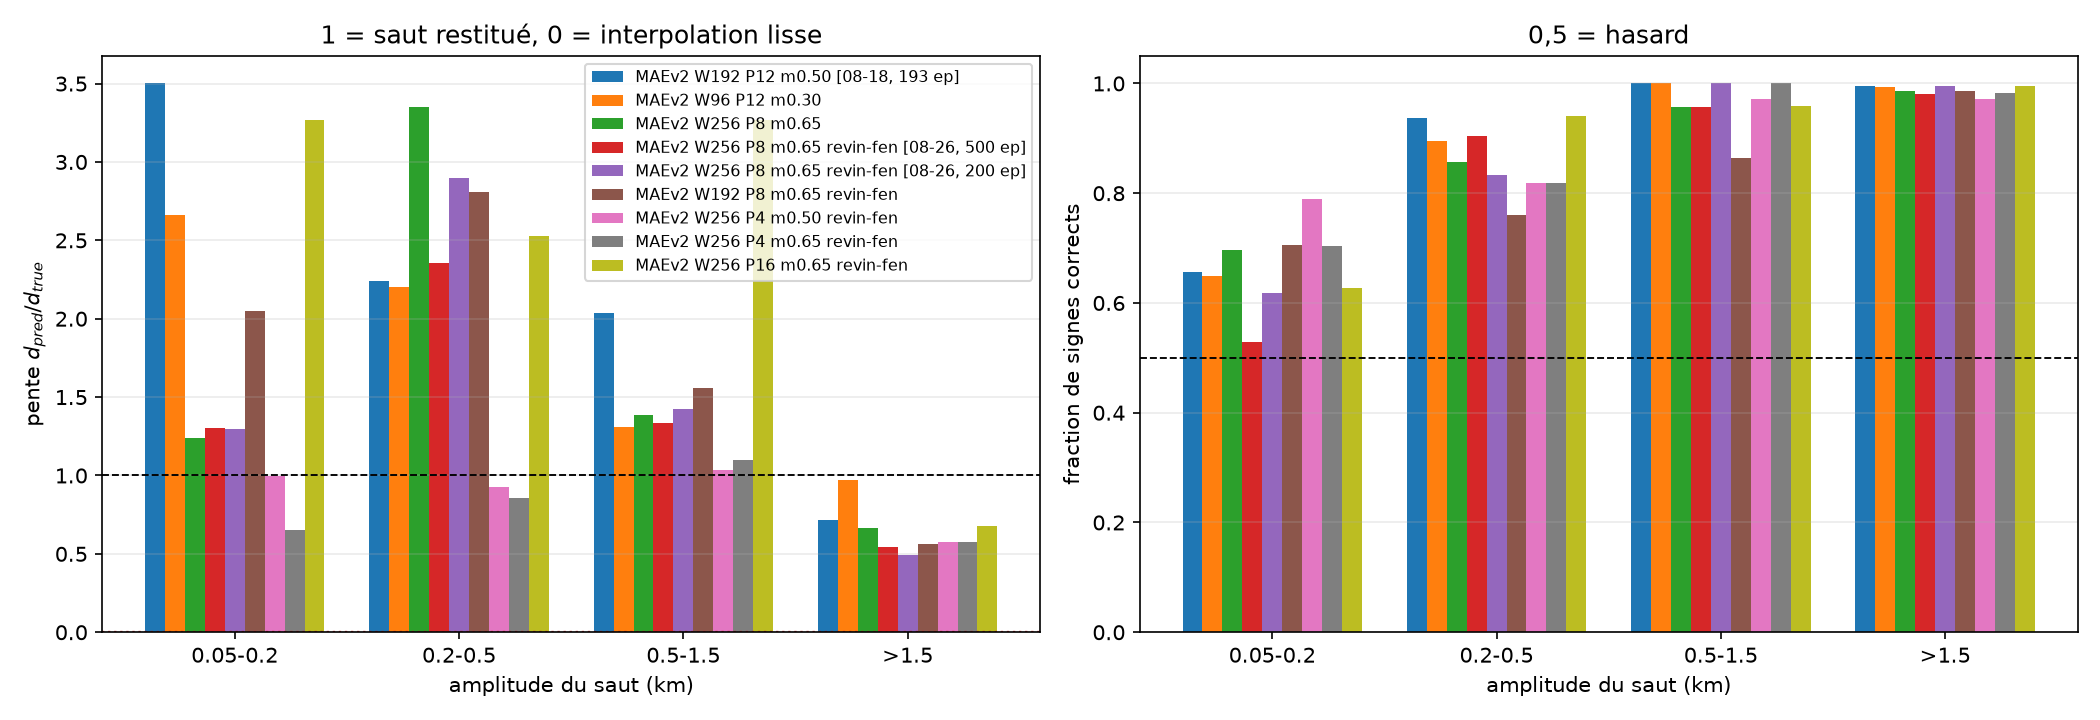
\includegraphics[width=0.98\textwidth]{figures/pretrain_leo_steps.png}
\end{center}

Les deux réserves de la section 4.7 s'appliquent : $\beta$ est atténué par le bruit sur la variable explicative, et sa valeur globale est dominée par les évènements de grande amplitude.

\subsection{Sonde linéaire et structure des embeddings}

$R^2$ en validation d'une régression ridge sur embedding gelé, cibles log-transformées, $2\,000$ objets dont $400$ en validation. Les trois premières colonnes sont des contrôles --- les grandeurs y sont directement présentes en entrée --- et les quatre suivantes des cibles dynamiques. Les deux dernières colonnes donnent le nombre de clusters HDBSCAN à hyperparamètres fixés et la fraction d'objets étiquetés bruit.

\begin{center}\tiny
\begin{tabular}{lccccccccc}
\toprule
Run & sma moyen & excentricite & inclinaison & derive sma & amplitude sma & taux de rupture & bruit propre & Clusters & Bruit \\
\midrule
MAEv2 W192 P12 m0.50 [08-18, 193 ep] & 0,97 & 0,96 & 0,98 & 0,90 & 0,89 & 0,75 & -0,16 & 8 & 0,25 \\
MAEv2 W96 P12 m0.30 & 0,90 & 0,94 & 0,99 & 0,94 & 0,92 & 0,78 & 0,45 & 8 & 0,26 \\
MAEv2 W256 P8 m0.65 & 0,98 & 0,95 & 0,99 & 0,88 & 0,92 & 0,80 & -0,67 & 7 & 0,28 \\
MAEv2 W256 P8 m0.65 revin-fen [08-26, 500 ep] & 0,93 & 0,86 & 0,97 & 0,91 & 0,93 & 0,92 & -2,34 & 8 & 0,41 \\
MAEv2 W256 P8 m0.65 revin-fen [08-26, 200 ep] & 0,95 & 0,90 & 0,96 & 0,93 & 0,93 & 0,84 & -1,45 & 8 & 0,35 \\
MAEv2 W192 P8 m0.65 revin-fen & 0,94 & 0,88 & 0,95 & 0,90 & 0,92 & 0,82 & -0,16 & 12 & 0,41 \\
MAEv2 W256 P4 m0.50 revin-fen & 0,96 & 0,86 & 0,92 & 0,95 & 0,95 & 0,91 & -0,70 & 12 & 0,44 \\
MAEv2 W256 P4 m0.65 revin-fen & 0,98 & 0,96 & 0,93 & 0,92 & 0,97 & 0,92 & 0,26 & 9 & 0,44 \\
MAEv2 W256 P16 m0.65 revin-fen & 0,95 & 0,90 & 0,97 & 0,94 & 0,95 & 0,90 & -1,57 & 9 & 0,42 \\
\bottomrule
\end{tabular}

\end{center}

\begin{center}
    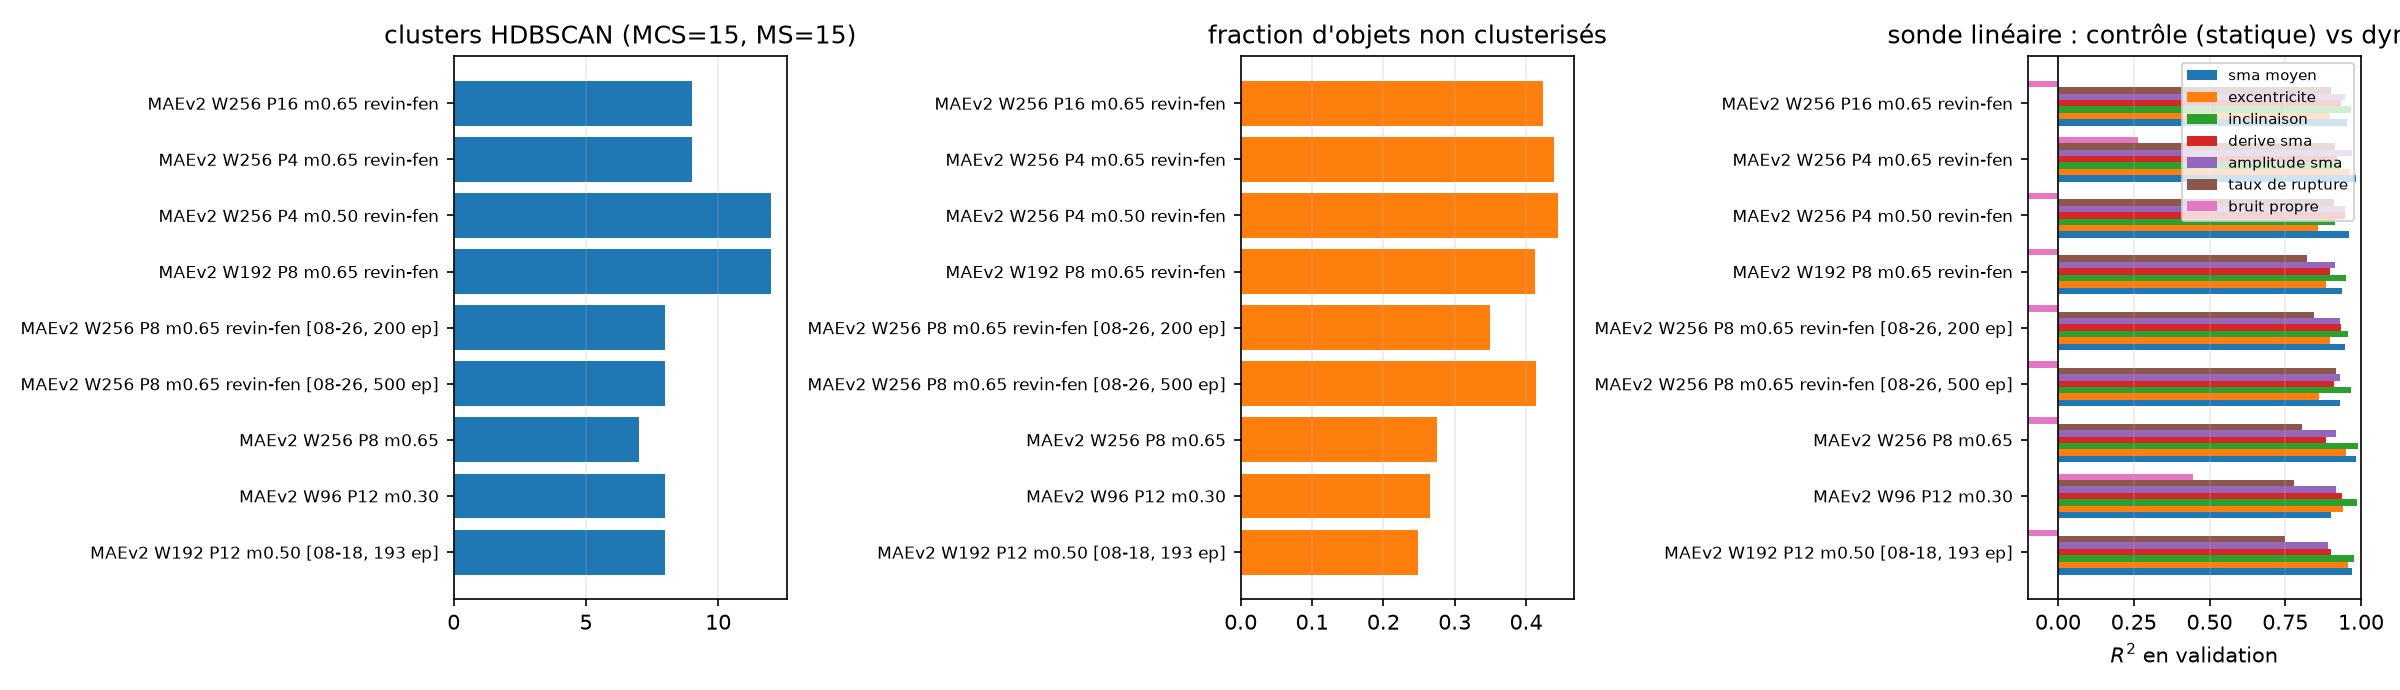
\includegraphics[width=0.98\textwidth]{figures/pretrain_leo_embeddings.png}
\end{center}

\paragraph{Lecture.} Sur les cibles de contrôle, tous les runs sont au-dessus de $R^2 = 0{,}90$. Sur les trois cibles dynamiques exploitables --- dérive, amplitude de variation et taux de rupture --- les $R^2$ s'échelonnent de $0{,}73$ à $0{,}95$ selon le run et la cible. Le \texttt{bruit propre} donne des valeurs comprises entre $-0{,}67$ et $+0{,}67$ selon les runs, sans ordre stable ; cette cible n'est pas exploitable en l'état.

\paragraph{Sur l'ordre des runs.} L'ordre des configurations selon la sonde n'est pas celui de la matrice de masquage : la configuration qui présente l'erreur de forme la plus faible n'est pas celle qui obtient les meilleurs $R^2$ dynamiques. Distinguer une différence réelle d'un effet d'échantillonnage demanderait de répéter la sonde sur plusieurs partitions train/validation, ce qui n'a pas été fait ici.

\subsection{Reconstructions}

Mêmes objets, mêmes fenêtres, mêmes patchs masqués, deux normalisations. Noir : série réelle. Rouge : reconstruction, tracée uniquement sur les patchs masqués.

\begin{center}
    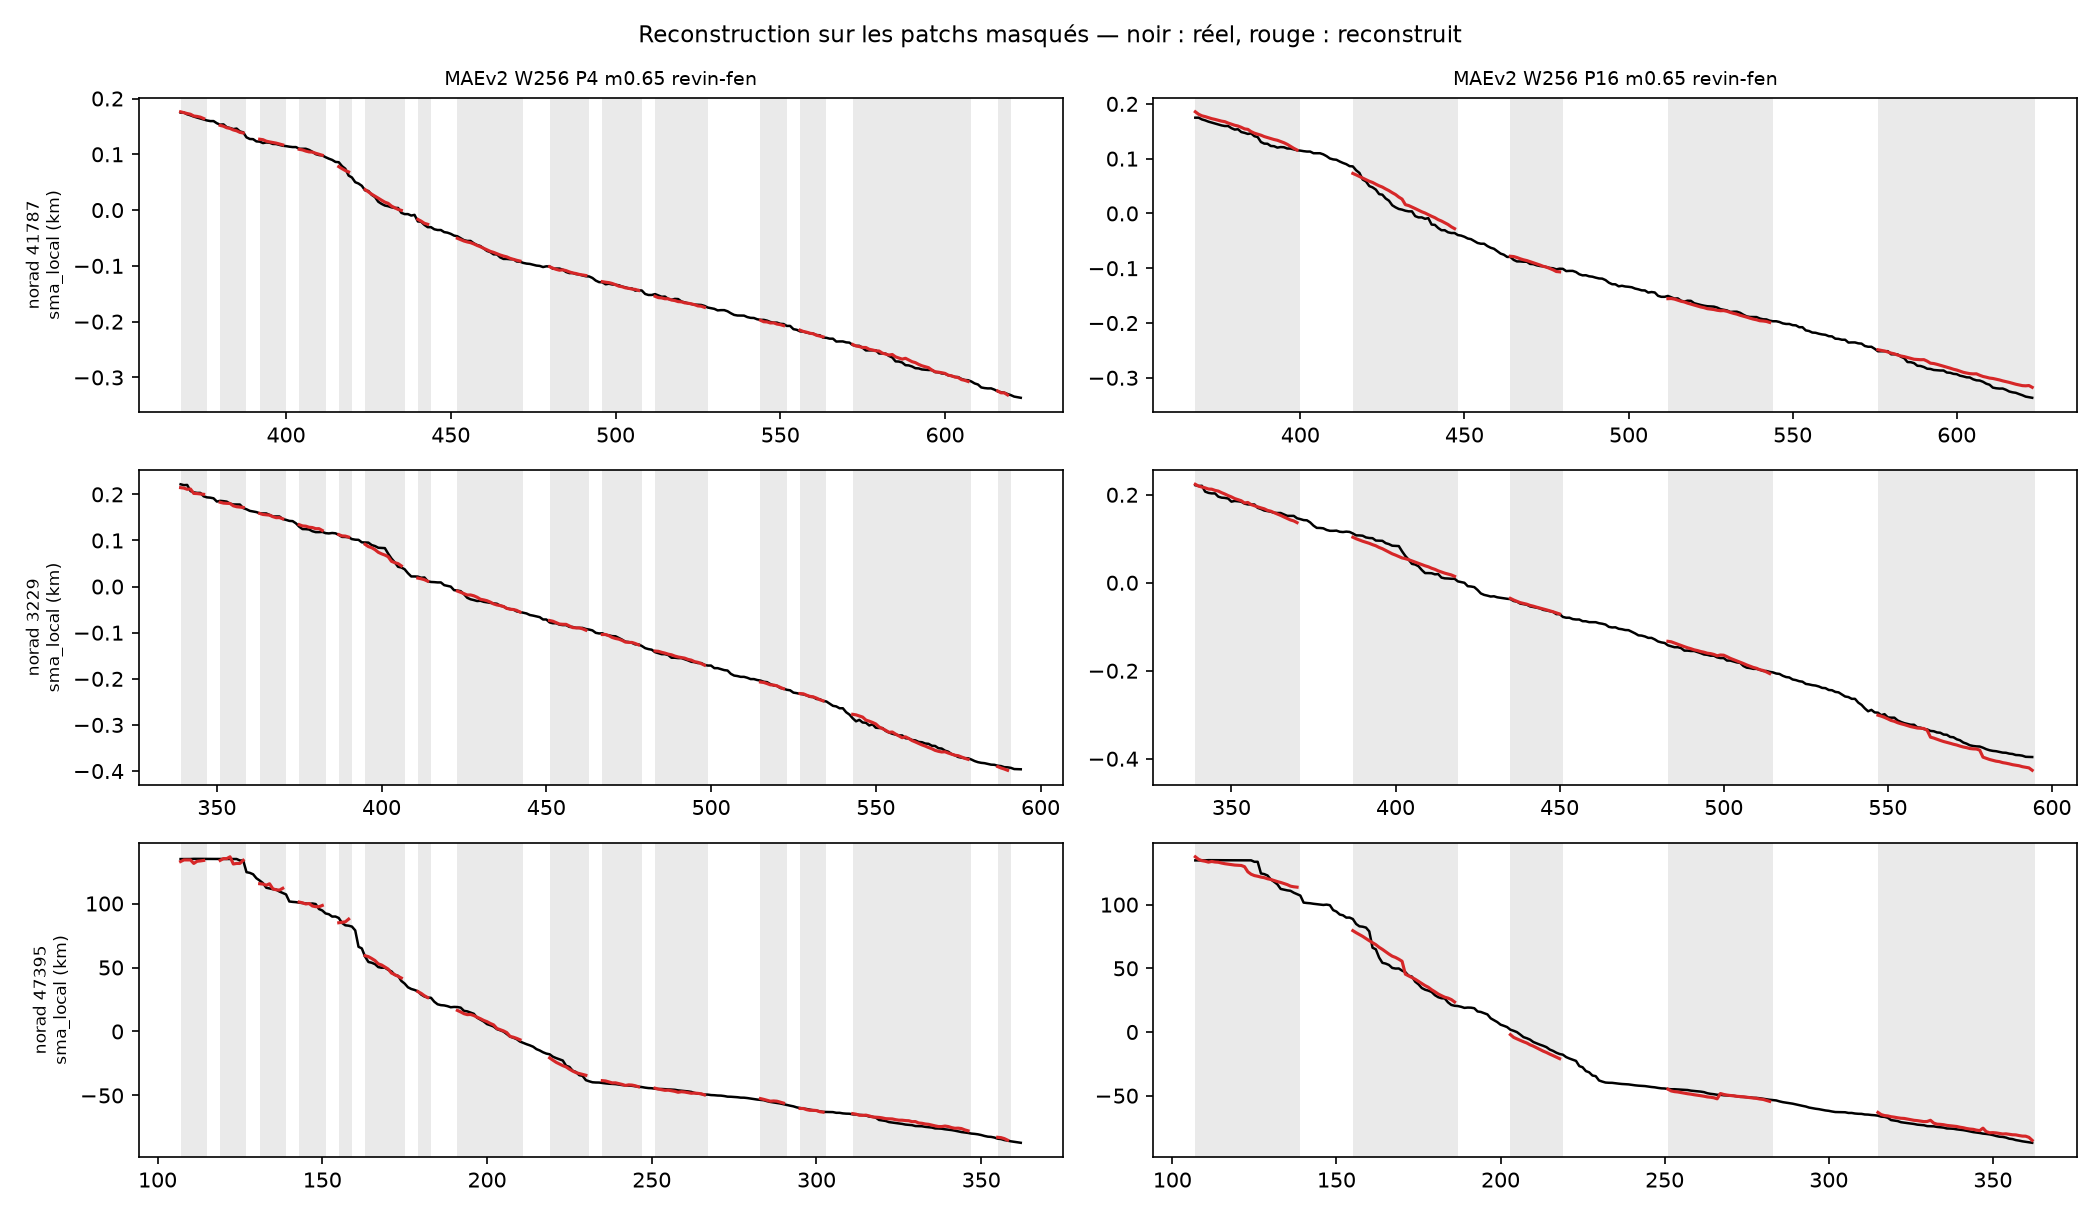
\includegraphics[width=0.98\textwidth]{figures/pretrain_leo_examples.png}
\end{center}

\section{Références}

\begin{thebibliography}{9}

\bibitem{he2022mae}
K.~He, X.~Chen, S.~Xie, Y.~Li, P.~Dollár, R.~Girshick.
\textit{Masked Autoencoders Are Scalable Vision Learners}. CVPR, 2022.

\bibitem{wang2023videomaev2}
L.~Wang, B.~Huang, Z.~Zhao, Z.~Tong, Y.~He, Y.~Wang, Y.~Wang, Y.~Qiao.
\textit{VideoMAE V2: Scaling Video Masked Autoencoders with Dual Masking}. CVPR, 2023.

\bibitem{nie2023patchtst}
Y.~Nie, N.~H.~Nguyen, P.~Sinthong, J.~Kalagnanam.
\textit{A Time Series is Worth 64 Words: Long-term Forecasting with Transformers}. ICLR, 2023.

\bibitem{kim2022revin}
T.~Kim, J.~Kim, Y.~Tae, C.~Park, J.-H.~Choi, J.~Choo.
\textit{Reversible Instance Normalization for Accurate Time-Series Forecasting against Distribution Shift}. ICLR, 2022.

\bibitem{broucke1972}
R.~A.~Broucke, P.~J.~Cefola.
\textit{On the equinoctial orbit elements}. Celestial Mechanics, 5(3), 1972.

\bibitem{vallado2008}
D.~A.~Vallado, P.~Crawford.
\textit{SGP4 Orbit Determination}. AIAA/AAS Astrodynamics Specialist Conference, 2008.

\bibitem{campello2013}
R.~J.~G.~B.~Campello, D.~Moulavi, J.~Sander.
\textit{Density-Based Clustering Based on Hierarchical Density Estimates}. PAKDD, 2013.

\end{thebibliography}

\end{document}
